%!TEX root=../../../main.tex

Most Web application nowadays include a social aspect, mostly in the shape of
message forums or commenting capabilities. Apart from platforms fully targeted
at communication among their users, such as message boards, other applications
include facilities that allow commenting the principal features, displayed
content, or simply facilitate the communication between users.  Notable
examples include most web blogs, which usually allow comments on post, YouTube,
which encourages users to discuss videos, or Facebook which augments the social
aspect by embedding comments on all the updates posted by its users.

An emerging trend among web applications is represented by the usage of the
social capabilities of one platform for augmenting another application or
website. For example, Facebook offers the possibility of embedding its widgets,
such that users can comment on external sources using their existing social
network accounts. A more full-fledged solution in this direction is Disqus
\cite{ref:disqus}, which provides commenting as a service to other
applications, as exemplified in Fig. \ref{fig:disqus}. Such solutions offer
advantages from the points of view of both the application provider and the end
user. The provider saves development time by not having to build a custom
commenting system, while users are given the opportunity to aggregate comments
and annotations generated across applications on various information resources.

\begin{figure}[!ht]
  \centering
  \fbox{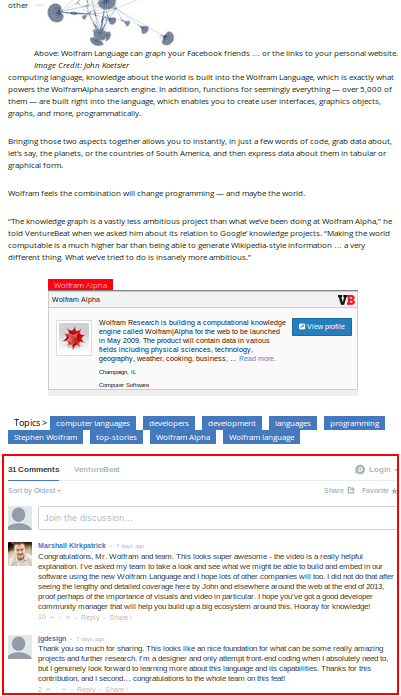
\includegraphics[scale=0.7]{static/img/disqus.png}}
  \caption[Disqus commenting widget embedded on a web blog]
          {Disqus commenting widget (highlighted in red rectangle) embedded on a web blog.}
  \label{fig:disqus}
\end{figure}

Most commenting solutions propose a plain text format for the inserted notes,
but alternatives exist. Rich text editors, such as CKEditor \cite{ref:cked} are
often used to allow standard formatting actions (e.g., bold text) on Web forms.
More customisation options can be implemented by using special markup, such as
XML or LaTeX, which is converted to the target format (e.g., HTML for Web
applications). Content structure can be enforced by implementing special forms
(see Inspire example in Fig. \ref{fig:inspire}) or by pre-defining constraints
for the users to follow when inserting plain text (see Section \ref{sec:data}
for an example).

While comments satisfy the needs of most applications in terms of social
interaction with and between the end users, they fall short in terms of adding
private notes or enriching existing content by augmenting it with
user-generated material. A trend among the Web community is related to
annotations, which are small pieces of information attached to various
resources, regardless of their type (images, (hyper)text, videos).

Kahan et al.\cite{ref:annotea} proposed the Annotea system, which allows adding
structured RDF notes on Web Documents. The annotations are viewed as statements
made by the author about the document. Annotea uses the Amaya \cite{ref:amaya}
editor on the frontend, and a generic RDF database accessible via HTTP server
for storage.

The Annotator project \cite{ref:annotator} allows developers to embed a special
widget on their web pages, in order to enable users to annotate any available
textual content, as exemplified in Fig. \ref{fig:annotator}.  It proposes a
JavaScript front-end, annotations being saved in the JavaScript Object Notation
format in order to be stored on the server side (the reference implementation
features a Python wrapper around Elasticsearch \cite{ref:elasearch}.

\begin{figure}[!ht]
  \centering
  \fbox{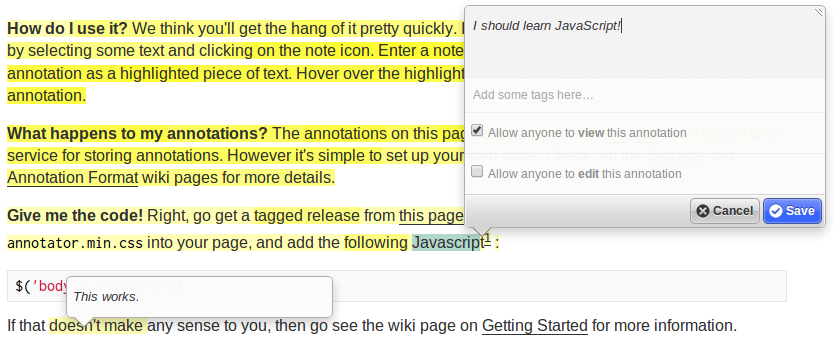
\includegraphics[scale=0.55]{static/img/annotator.png}}
  \caption[Example usage of the Annotator project]
          {Example usage of the Annotator project. It allows
           adding annotations on any Web page element; in this example, a form
           for annotating a piece of textual information is displayed.}
  \label{fig:annotator}
\end{figure}

While the Annotator project provides a limited number of features, it has an
open plugin interface, which allows third-parties to provide various additions,
such as an image tagging facility, an offline editing mode, or various
visualisation utilities. It is interesting to note that, in contrast to the
commenting solution discussed previously, this project regards private
annotations as first-class citizens, support for shared content being provided
only via a plugin. While the main purpose of the system is to be deployed over
existing applications, a stand-alone version which allows users to keep a
record of annotations over any Web resource is also provided.

A similar project, funded by the European Union's Seventh Framework Programme,
is Pundit \cite{ref:pundit}, which was initially developed in order to enable
humanities researchers to work with manuscripts by leveraging linked data.
Similar to Annotator, it features a JavaScript interface that allows users to
annotate any Web page, but it provides more features in terms of formatting and
structuring the annotations. For example, it allows generating RDF triples, as
exemplified in Fig. \ref{fig:pundit}.

\begin{figure}[!ht]
  \centering
  \fbox{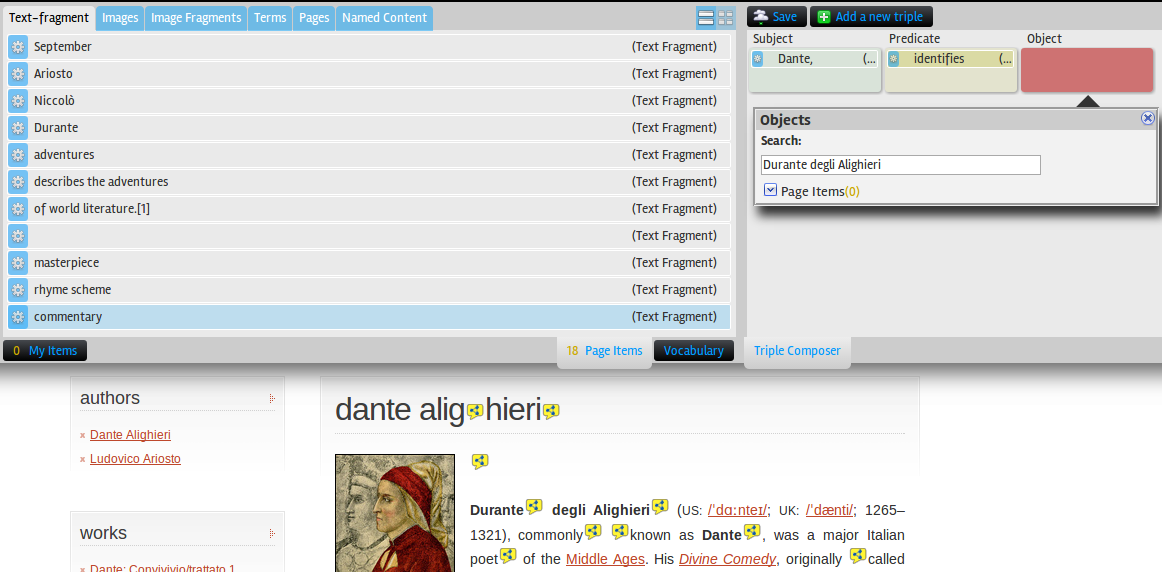
\includegraphics[scale=0.28]{static/img/pundit.png}}
  \caption[Example usage of the Pundit project]
          {Example usage of the Pundit project. Alike Annotator, it allows
           inserting annotations into Web pages, featuring a rich editor
           including RDF triples creation support (right hand side.}
  \label{fig:pundit}
\end{figure}

The main focus of Pundit is allowing users to collaboratively build a knowledge
graph, annotations being targeted not only at augmenting Web pages with
confined information, but also at linking various resources residing on
different domains.

Pundit is designed as a client-server application. The JavaScript client
communicates with the backend via an exposed REST\footnote{See Section
\ref{sec:pub} for more details regarding the REST architecture.} interface,
which can also be used by third party plugins. Annotations are stored in a RDF
triple store which exposes a standard SPARQL \cite{ref:sparql} endpoint. The
open nature of the software facilitates the extension of the platform; for
example, video resource tagging was implemented into Pundit
\cite{ref:punditvideo}.

It is important to note that between Annotea and newer projects such as
Annotator and Pundit, the community seemed to move from defining a strict
structure for annotations to a more loose format or to even dropping any
content restrictions. While this might impede the consumption of annotations by
automated systems, it also makes the process more accessible to users allowing
for more metadata to be collected, better reflecting the web resources' meaning
from the users' point of view\cite{ref:wu}.
